%-----------------------------------------------------------------------------%
%                                                                             %
%    K A P I T E L   2                                                        %
%                                                                             %
%-----------------------------------------------------------------------------%

\chapter{Mathematical Background: Optimal Bipedal Locomotion}\label{c2}
The second chapter provides the reader with fundamentals regarding terminology, modeling and stability analysis in the context of humanoid robotics and presents the class of used algorithms with its relevant extensions used in the context of this thesis.

\section{Foundations of Bipedal Locomotion}\label{sec:TheoryBiped}
\subsection{Terminology}
In order to describe the locomotion of a humanoid robot, specific terms are required that are introduced within this section. \citeauthor{vukobratovic2007towards} provide an extensive introduction to the terminology related to bipedal walking \cite{vukobratovic2007towards}, concisely summarized by \citeauthor{dekker2009zero} \cite{dekker2009zero}.\\\\
\textbf{Walk}\\
Walk can be defined as: ``\textit{Movement by putting forward each foot in turn, not having both feet off the ground at once}''.\\\\
\textbf{Run}\\
Run is characterized by both feet partially leaving the ground at the same time.\\\\
\textbf{Gait}\\
The way each human walks and runs is unique, hence gait can be defined as: ``\textit{Manner of walking or running}''.\\\\
\textbf{Periodic gait}\\
If a gait is realized by repeating each locomotion phase in an identical 
\footnote{The locomotion phase can be identical w.r.t. the step size or the duration, depending on the index.} way, the gait is referred to as \textit{periodic}.\\\\
\textbf{Symmetric gait}\\
If the left and right leg move in an identical but time-shifted manner, the gait is referred to as \textit{symmetric}.\\\\
\textbf{Double Support}\\
A situation where the humanoid has two isolated contact surfaces with the ground.\\\\
\textbf{Single Support}\\
A situation where  the humanoid has only one contact surface with the ground.\\\\
\textbf{Support Polygon}\\%TODO: Maybe add figure to illustrate single vs double support
The support polygon is formed by the \textit{convex hull} about the ground contact points.    \\\\
\textbf{Swing foot}\\
This term refers to the leg that is performing a step, i.e. moving through the air.\\\\
\textbf{Supporting foot}\\
This term refers to the leg that is in contact with the ground, supporting all the weight of the humanoid. 

\subsection{Dynamic Modeling of Legged Robots}\label{subsec:DynamicModeling}
In the following, the dynamic model for floating base systems, such as legged robots, is derived based on a general formulation. A concise introduction to dynamic modeling is presented with \cite{scaronTeaching}, comprehensive studies can be found in \cite{pfeiffer1996multibody, jain2010robot, featherstone2014rigid}.
\subsubsection{General Formulation}
Mathematical models of a robot's dynamics describe the motion as a function of time and control inputs. These models are the basis for both simulation and control of robotic systems. In an abstract form, the \gls{EoM} can be written as: 
\begin{equation} \label{eqn:EoMGeneral}
F(\bq(t),\bdq(t),\bddq(t),\bu(t),t)=0,
\end{equation}
where 
\begin{itemize}
\item $\bt$ is the time variable, 
\item $\bq$ is the vector of generalized coordinates,
\item $\bdq$ is the first time derivative (velocity) of \bq, 
\item $\bddq$ is the second time derivative (acceleration) of \bq and
\item $\bu$ is the vector of control inputs. 
\end{itemize}
Consequently, the \gls{EoM} provide a mapping between the control space on the one hand and the state space of robot on the other hand. Typical methods for computing the closed-form solution of the \gls{EoM} are e.g. the classical \textit{Newton-Euler} \cite{luh1980line} method or the \textit{Lagrange method} \cite{hollerbach1980recursive}, where the former is based on principles for conservation of linear and angular momenta and the latter utilizes energy-based functions expressed in generalized coordinates. 
\subsubsection{Fixed Base Systems}
For applications with fixed-based robots, e.g. a robotic manipulator, the multi-body dynamics can be formulated as
\begin{equation} \label{eqn:EoMManipulator}
\myM{M}(\bq)\bddq+\bdq^T\myM{C}(\bq)\bdq=\btau+\btau_g(\bq),
\end{equation}
where 
\begin{itemize}
\item $\myM{M}(\bq)$ is the generalized inertia matrix, 
\item $\myM{C}(\bq)$ is the coriolis tensor, 
\item $\btau$ is the vector of actuated joint torques and 
\item $\btau_g(\bq)$ is the vector of external joint torques caused by gravity.
\end{itemize}
In contrast to the general formulation in \cref{eqn:EoMGeneral}, this expression is time-invariant. Hence, \cref{eqn:EoMManipulator} can be used for computing the \gls{FD}, as well as the \gls{ID} of a robotic system.

\subsubsection{Implicit and Explicit Constraints}
%Why constrains?
The motion of a robot is constrained by it's kinematics structure as well as additional constraints that may arise from the environment. \cref{img:constraints} provides a classification of kinematic constraints, which are often found in the field of robotics \cite[Ch.3]{kumar2019modular}. While equality constraints arise from permanent physical contact between two bodies, inequality constraints arise due to phenomena such as collision, bouncing or loss of contact. Equality constraints can be further divided into holonomic and non-holonomic constraints. The former constrain the position (e.g. fixed or sliding contacts), the latter constrain the velocity (e.g. rolling contacts) of multi-body systems. 

\begin{figure}
\centering	
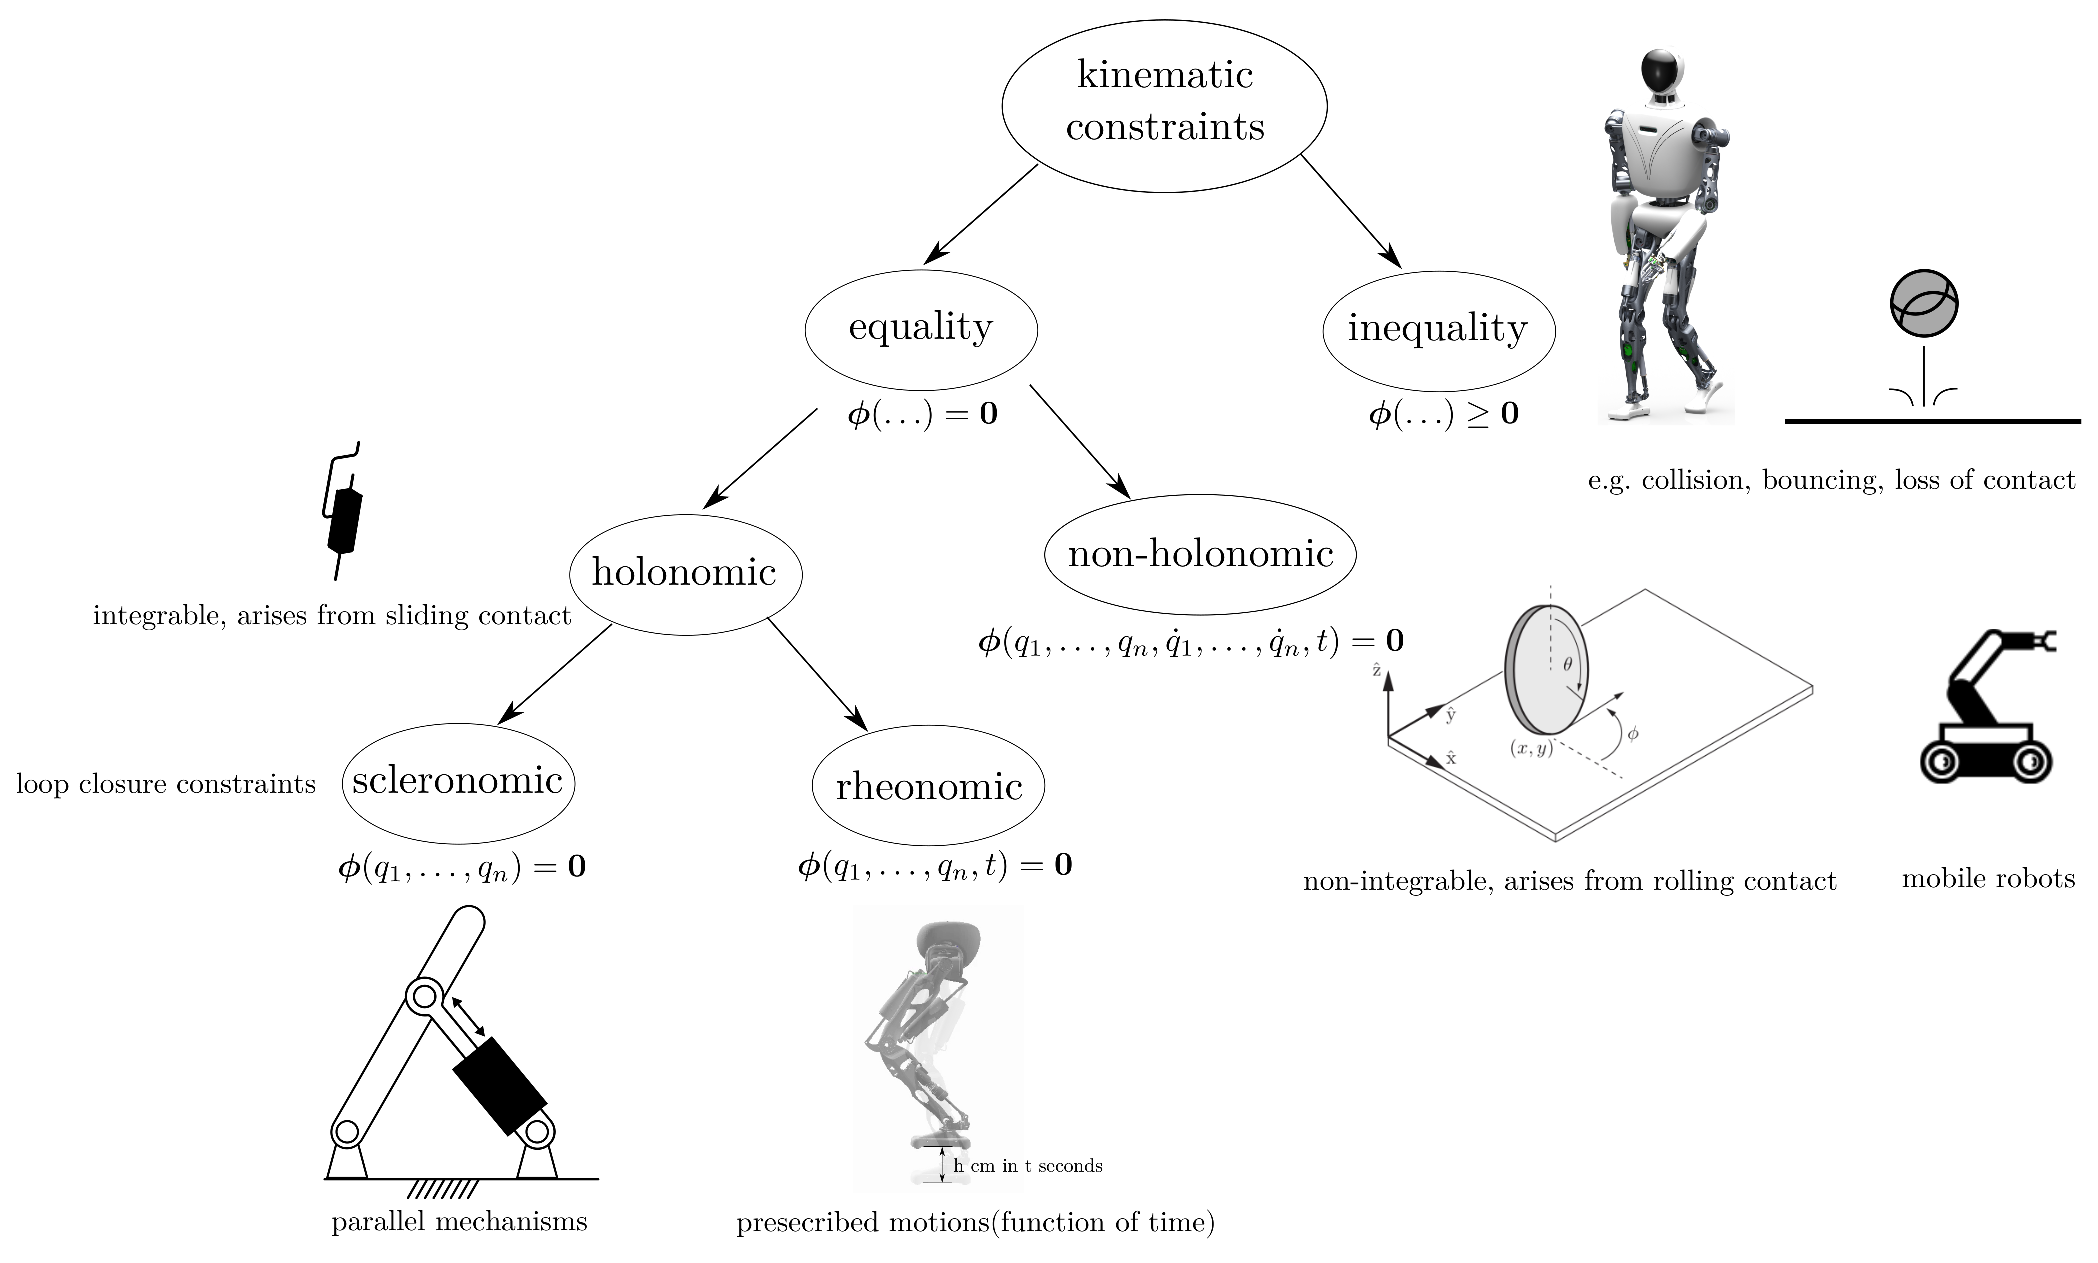
\includegraphics[width=1\textwidth]{img/constraints}
\caption[Kinematic constraints in multi-body systems]{Classification of kinematic constraints in multi-body systems \cite{kumar2019modular}.}
\label{img:constraints}
\end{figure} 

In the scope of this thesis, we focus on mobile robots that contain parallel mechanisms. In contrast to serial manipulators, two additional scleronomic constraints have to be actively enforced for this type of robotic systems:
\begin{itemize}
\item Internal loop closure constraints,
\item Contact constraints.
\end{itemize}

The contact constraints are  modeled explicitly as holonomic scleronomic constraints in the robot dynamics (see \cref{subsec:DDPConstrainedRobotDynamics}). Since the dynamics solvers inside Crocoddyl do not allow computation for series-parallel mechanisms, a serialized robot model is used as basis of the \gls{OC} problem. Hence, the closed loop constraints are only implicitly considered within the control architecture (see \cref{subsec:Pipeline}). Although the usage of this simplified model reduces the accuracy, it is proven to be sufficient for dynamic real-time control \cite{kumar2019model}.

\subsubsection{Floating Base Systems}
As previously mentioned, the focus of this thesis is on mobile robots. These so-called floating base systems are characterized by having a base that is free to move, rather than being fixed in space. Consequently, the vector of generalized coordinates $\bq$ not only contains the joint's angles, but also accounts for the position and orientation of the floating base. Legged robots belong to this category of rigid-body systems as they make and break contacts with their environment in order to move. Contrary to manipulators, contacts need to be actively enforced by holonomic constraints for legged robots. There are namely two different types of contact constraints that can be applied: point contacts (3D) or surface contacts (6D). 

For the case of point contacts, the dynamics of the floating base system become
\begin{equation*} \label{eqn:EoMLeggedRobotPtContact}
\myM{M}(\bq)\bddq+\bdq^T\myM{C}(\bq)\bdq=\myM{S}^T\btau+\btau_g(\bq)+\sum_{i=1}^{k}\myM{J}_{C_i}^T\bfun_i,
\end{equation*}
where 
\begin{itemize}
\item \myM{S} is the selection matrix of actuated joints,
\item $\myM{J}_{C_i}$ is the Jacobian at the location of a contact point $C_i$ and
\item $\bfun_i$ is the contact force acting at the contact point $C_i$.
\end{itemize}
For the case of surface contacts, such as a flat foot on a flat floor, modeling a point contact is not sufficient since it only constrains the translation. In order to also account for the rotational constraints enforced by the geometry one could take into account multiple point contacts. A non-redundant alternative is to model more general frame contact constraints as
\begin{equation} \label{eqn:EoMLeggedRobotSurfaceContact}
\myM{M}(\bq)\bddq+\bdq^T\myM{C}(\bq)\bdq=\myM{S}^T\btau+\btau_g(\bq)+\sum_{i=1}^{k}\myM{J}_{C_i}^T\myM{w}_i,
\end{equation}
where $\myM{w}_i$ is referred to as the \textit{contact wrench} acting on the contact link $i$. This wrench stacks the resulting $\bfun_i$ of contact forces and the moment $\btau_i$ exerted by these forces around the contact frame as
$$\myM{w}_i=(\bfun_i,\btau_i)_{6\times 1}.$$ 
For more details on contact wrenches and spatial vector algebra in general, the interested reader is referred to e.g. \cite[Ch.2]{featherstone2014rigid}.


\section{Stability Analysis: Not Falling Down}\label{sec:TheoryStability}
Humanoid robots are high-dimensional, constrained and nonlinear dynamical systems. In this section, the most common criteria  for analyzing the long-term stability behavior of such complex systems are presented. Exhaustive studies on stability criteria and their relation can be found in \cite{garcia2002classification, dekker2009zero, siciliano2016springer}.

\subsection{Static Stability Criteria}
\subsubsection{Floor Projection of the Center of Mass (FCoM)}
Consider the case of a robot that is not moving, i.e. a humanoid in static double support. In that case, the only forces acting on the humanoid are the ones caused by gravity. These forces can be represented by a virtual force acting on the \gls{CoM} of the robot. The position of the \gls{CoM} w.r.t. the base frame can be described by
\begin{equation*} 
\bp_{\text{CoM}}=\dfrac{\sum_{i=1}^{n}m_i\bp_i}{\sum_{i=1}^{n}m_i},
\end{equation*}
where the robot has $n$ links and $\bp_i$ indicate the according link distances of the individual \gls{CoM}s. The \gls{FCoM} equals the first two components of the \gls{CoM} position vector $\bp_{CoM}$ and the following relation holds:
\begin{equation*} 
\sum_{i=1}^{n}((\bp_{\text{FCoM}}-\bp_i)\times m_i\bg)=\myM{0}.
\end{equation*}
The \gls{FCoM} can be used as a static stability margin, ensuring the motionless robot will not tip over or fall, if $\bp_{\text{FCoM}}$ always remains inside the \gls{SP}. Note that this criteria is also applicable in so called \textit{quasi-static} movements, where static forces are still dominating dynamic forces.

\subsection{Dynamic Stability Criteria}
In case of faster motions, dynamic forces will exceed the static forces and cannot be neglected anymore. The acting forces can be divided into contact forces and gravity/inertial forces, where the so called \gls{ZMP} is based on the former, and the \gls{CoP} on the latter. In the following, both concepts are introduced according to the description in \cite{sardain2004forces} with a nomenclature equivalent to \cite{scaronTeaching}.
\subsubsection{Center of Pressure (CoP)}
The \gls{CoP} is defined as the point, where the field of pressure forces acting on the sole is equivalent to a single resulting force where the resulting moment is zero. Hence the \gls{CoP} is a local quantity that is derived from the interaction forces at the contact surface. 

Considering the case of a foot contacting a plane surface, the resulting contact force $\bfun^c$ is exerted by the environment onto the robot. This force consists of the resulting pressure force $\bfun^p=(\bfun^c\cdot\bn)\bn$, as well as the resulting friction force ${\bfun^f=\bfun^c-\bfun^p}$.
Hence, the following conditions hold:
\begin{align*}
\btau_O^p 		&= \myM{0} \\
\bp_{\text{CoP}}\times(\bfun^p\cdot\bn)\bn	&= -\btau_O^P \\
(\bfun^p\cdot\bn)\bn\times\bp_{\text{CoP}}\times\bn	&= -\bn\times\btau_O^p
\end{align*}
Since both the sole point $O$ and $\bp_{\text{CoP}}$ belong to the same plane, we get:
\begin{equation*}
\bp_{\text{CoP}}=\dfrac{\bn\times\btau_O^p}{\bfun^p\cdot\bn}.
\end{equation*}
Finally, friction forces are tangent to the contact surface and their moment is aligned with $\bn$, so we equivalently can write this relationship as:
\begin{equation}\label{eqn:CoPComputation}
\bp_{\text{CoP}}=\dfrac{\bn\times\btau_O^c}{\bfun^c\cdot\bn}.
\end{equation}
\Cref{eqn:CoPComputation} can be used to compute the \gls{CoP} expressed in the local contact frame.

%\begin{figure}[h!]
%\centering	
%\includegraphics[width=.5\textwidth]{img/CoP1}
%\caption{}
%\label{img:rh5_robot}
%\end{figure} 
%
%\begin{figure}[h!]
%\centering	
%\includegraphics[width=.6\textwidth]{img/CoP2}
%\caption{}
%\label{img:rh5_robot}
%\end{figure} 
\subsubsection{Zero-Moment Point (ZMP)}
The \gls{ZMP} is defined as a point on the ground where the \textit{tipping moment} acting on the biped equals zero. This condition can be interpreted as a constraint on the contact moments, which contains at least the roll and pitch direction. Originally, the concept has been introduced in \cite{vukobratovic1972stability}, it has been reviewed in \cite{vukobratovic2004zero} and made popular with \cite{kajita2003biped}.

The concept is build upon two key assumptions:
\begin{itemize}
\item There exists one planar contact surface (i.e. no multiple surfaces like on rough terrain)
\item The friction is sufficiently high to prevent sliding of the feet
\end{itemize}
From the Newton-Euler equations, the motion of the biped can be written as
\begin{align*}
m\ddot{\bp}_{\text{CoM}} &= m\bg+\bfun^c \\
\dot{\myM{L}}_O &= \bp_{\text{CoM}}\times m\bg+\btau_{\text{CoM}}^c,
\end{align*}
where $m$ denotes the total mass of the robot, $\bg$ is the gravity vector, $\ddot{\bp}_{\text{CoM}}$ the centroidal acceleration, $\dot{\myM{L}}_O$ the change of the angular momentum. $\bw_{\text{CoM}}^c=(\btau_{\text{CoM}}^c, \bfun^c)_{6\times 1}$ denotes the sum of all contact wrenches in the \gls{CoM} frame. The gravito-inertial wrench of the robot can be defined as
\begin{align*}
\bfun^{gi} &= m(\bg-m\ddot{\bp}_{\text{CoM}}) \\
\btau_O^{gi} &= \bp_{\text{CoM}}\times m\bg-\dot{\myM{L}}_O.
\end{align*}
Using the wrench form of the Newton-Euler equations
\begin{equation}\label{eqn:NewtonEuler} 
\bw^{gi}+\bw^c=\myM{0},
\end{equation}
one can derive the \gls{ZMP}, for the case of a planar surface, as
\begin{equation}\label{eqn:ZMPComputation}
\bp_{\text{CoM}}=\dfrac{\bn\times\btau_O^{gi}}{\bfun^{gi}\cdot\bn}.
\end{equation}
In practice, one can use this formula to compute the \gls{ZMP} from force sensors or from an inertial measurement unit. 
\subsubsection{Coincidence of ZMP and CoP}
As \citeauthor{sardain2004forces} outline, both the \gls{ZMP} and the \gls{CoP} yield the same point for the case of bipedal walking on a single plane surface \cite{sardain2004forces}. Comparing \cref{eqn:ZMPComputation} with \cref{eqn:CoPComputation}, we recognize the only difference is that the former is applied to the (global) gravito-inertial wrench, while the latter is applied to the (local) contact wrench. If we recall the Newton-Euler equations from \cref{eqn:NewtonEuler}, it becomes clear why both points coincide when there is only one contact plane.

\subsection{Stability Classification}
There are existing several classifications of stability, which will be defined in the following according to \cite[Sec.1.2.1]{westervelt2018feedback} and \cite{garcia2002classification}. See \citeauthor{vukobratovic2007towards} for more details on differentiating the terms dynamic stability and dynamic balance \cite{vukobratovic2007towards}.  
\subsubsection{Statically Stable Motion}
The gait or movement of a humanoid is classified as \textit{statically stable} if the \gls{FCoM} does not leave the \gls{SP} during the entire motion or gait. Consequently, the humanoid will remain in a stable position, whenever the movement is stopped. Typically, these kinds of stability are only obtained with very low walking velocities or quasi-static motions, where the static forces dominate the dynamic forces. To this end, the \gls{FCoM} stability criteria is used for the generation of balanced static walking gaits (see \cref{sec:BipedSimulation}).   
\subsubsection{Dynamically Stable Motion}
If the \gls{FCoM} partially leaves the \gls{SP} at some point during the gait, but the \gls{CoP} (or \gls{ZMP}) always remains within the \gls{SP}, the gait or movement is classified as \textit{dynamically stable}. This stability margin is extremely useful for flat-foot dynamic walking since it prevents the foot from rotating around the boundary of the \gls{SP}. The \gls{CoP} is a central building block of the contact stability constrained \gls{DDP} approach that will be discussed in \cref{c3}.   


\section{Differential Dynamic Programming (DDP)}\label{sec:TheoryDDP}
This section describes the basics of \gls{DDP}, which is an \gls{OC} algorithm that belongs to the \gls{TO} class. The algorithm was introduced in 1966 by \citeauthor{mayne1966} \citep{mayne1966}. A modern description of the algorithm using the same notations as below can be found in \cite{tassa2012synthesis, tassa2014control}.
\subsection{Finite Horizon Optimal Control}
We consider a system with discrete-time dynamics, which can be modeled as a generic function $\bfun$
\begin{equation}\label{eqn:discreteDynamics}
\bx_{i+1}=\bfun(\bx_i,\bu_i), 
\end{equation}
that describes the evolution of the state $\bx\in \myM{R}^n$ from time $i$ to $i+1$, given the control $\bu\in \myM{R}^m$. A complete trajectory $\{\bx, \bu\}$ is a sequence of states $\bx=\{\bx_0, \bx_1, ..., \bx_N\}$ and control inputs $\bu=\{\bu_0, \bu_1, ..., \bu_N\}$ satisfying \cref{eqn:discreteDynamics}.
The \textit{total cost} $J$ of a trajectory can be written as the sum of running costs $l$ and a final cost $l_f$ starting from the initial state $\bx_0$ and applying the control sequence $\bu$ along the finite time-horizon:     
\begin{equation}\label{eqn:totalCost}
J(\bx_0, \bu)=l_f(\bx_N)+\sum_{i=0}^{N-1}l(\bx_i,\bu_i).
\end{equation}
As discussed in \cref{c1}, \textit{indirect} methods such \gls{DDP} represent the trajectory implicitly solely via the optimal control inputs $\bu$. The states $\bx$ are obtained from forward simulation of the system dynamics, i.e. integration \cref{eqn:discreteDynamics}. Consequently, the solution of the optimal control problem is the minimizing control sequence 
\begin{equation*}\label{eqn:minControl}
\bu^*=\argmin_U J(\bx_0, \bu). 
\end{equation*}

\subsection{Local Dynamic Programming}
Let $\bu_i\equiv\{\bu_i,\bu_{i+1}...,\bu_{N-1}\}$ be the partial control sequence, the \textit{cost-to-go} $J_i$ is the partial sum of costs from $i$ to $N$: 
\begin{equation}\label{eqn:costToGo}
J_i(\bx, \bu_i)=l_f(\bx_N)+\sum_{j=i}^{N-1}l(\bx_j,\bu_j).
\end{equation}
The \textit{Value function} at time $i$ is the optimal cost-to-go starting at $\bx$ given the minimizing control sequence 
\begin{equation*}\label{eqn:value}
V_i(\bx)=\min_{\bu_i}J_i(\bx, \bu_i),
\end{equation*}
and the Value at the final time is defined as $V_N(\bx)\equiv l_f(\bx_N)$. The Dynamic Programming Principle \citep{bellman1966dynamic} reduces the minimization over an entire sequence of control inputs to a sequence of minimizations over a single control, proceeding backwards in time: 
\begin{equation}\label{eqn:bellman}
V(\bx)=\min_{\bu}[l(\bx, \bu)+V'(\bfun(\bx,\bu))].
\end{equation}
Note that \cref{eqn:bellman} is referred to as the \textit{Bellman equation} for \textit{discrete-time} optimization problems \citep{kirk2004optimal}. For reasons of readability, the time index $i$ is omitted and $V'$ introduced to denote the Value at the next time step. The interested reader may note that the analogous equation for the case of \textit{continuous-time} is a partial differential equation called the \textit{Hamilton-Jacobi-Bellman equation} \citep{underactuatedCourse2020, kamien2012dynamic}.

\subsection{Quadratic Approximation}
\gls{DDP} locally computes the optimal state and control sequences of the \gls{OC} problem derived with \cref{eqn:bellman} by iteratively performing a forward and backward pass. The \textit{backward pass} on the trajectory generates a new control sequence and is followed by a \textit{forward pass} to compute and evaluate the new trajectory.

Let $\bQ(\dx,\du)$ be the variation in the argument on the right-hand side of \cref{eqn:bellman} around the $i^{th} (\bx,\bu)$ pair
\begin{equation}\label{eqn:Q}
\bQ(\dx,\du)=l(\bx+\dx,\bu+\du)+V'(\bfun(\bx+\dx,\bu+\du)).
\end{equation}
The \gls{DDP} algorithm uses a quadratic approximation of this differential change. The quadratic Taylor expansion of $Q(\dx,\du)$ leads to
\begin{equation}\label{eqn:QApprox}
\bQ(\dx,\du) \approx \dfrac{1}{2} 
\begin{bmatrix} 1 \\ \dx \\ \du \end{bmatrix}^T 
\begin{bmatrix} 0 & \bQ_{x}^T & \bQ_{u}^T \\
\bQ_{x} & \bQ_{xx} & \bQ_{xu} \\
\bQ_{u} & \bQ_{ux} & \bQ_{uu} \end{bmatrix}
\begin{bmatrix} 1 \\ \dx \\ \du \end{bmatrix}.
\end{equation}
The coefficients can be computed as  
\begin{subequations}\label{eqn:QApproxCoeff}
\begin{align}
\bQ_{x} &= l_{x}+\bfun_{x}^T \bV_{x}^\prime, \\
\bQ_{u} &= l_{u}+\bfun_{u}^T \bV_{x}^\prime, \\
\bQ_{xx} &= l_{xx}+\bfun_{x}^T \bV_{xx}^\prime\bfun_{x}+\bV_{x}^\prime\bfun_{xx}  \label{subeqn:Qxx},\\
\bQ_{ux} &= l_{ux}+\bfun_{u}^T \bV_{xx}^\prime\bfun_{x}+\bV_{x}^\prime\bfun_{ux} \label{subeqn:Qux},\\
\bQ_{bu} &= l_{uu}+\bfun_{u}^T \bV_{xx}^\prime\bfun_{u}+\bV_{x}^\prime\bfun_{uu} \label{subeqn:Quu}.
\end{align}
\end{subequations}
where the primes denote the values at the next time-step.  

\subsection{Algorithmic Steps}
%\subsubsection{Backward Pass}
The first algorithmic step of \gls{DDP}, namely the backward pass, involves computing a new control sequence on the given trajectory and consequently determining the search direction of a a step in the numerical optimization. To this end, the quadratic approximation obtained from \cref{eqn:QApprox}, minimized with respect to $\du$ for some state perturbation $\dx$, results in
\begin{equation*}
\du^*(\dx)=\argmin_{\du}\bQ(\dx,\du)=-\bQ_{uu}^{-1}(\bQ_{u}+\bQ_{ux}\dx),
\end{equation*}
giving us an open-loop term $\myM{k}$ and a feedback gain term $\bk$:
\begin{equation*}
\bk=-\bQ_{uu}^{-1}\bQ_{u}\quad \text{and} \quad \bk=-\bQ_{uu}^{-1}\bQ_{ux}.
\end{equation*}
The resulting locally-linear feedback policy can be again inserted into \cref{eqn:QApprox} leading to a quadratic model of the Value at time $i$: 
\begin{align*}
 \Delta \bV &= -\dfrac{1}{2}\bk^T\bQ_{uu}\bk \\
 \bV_{x} &= \bQ_{x}-\bk^T\bQ_{uu}\bk \\
 \bV_{xx} &= \bQ_{xx}-\bk^T\bQ_{uu}\bk.
\end{align*}

%\subsubsection{Forward Pass}
After computing the feedback policy in the backward pass, the forward pass computes a corresponding trajectory by integrating the dynamics via
\begin{align*}
\hat{\bx}_0 		&=\bx_0 \\
\hat{\bu}_i 		&=\bu_i+\alpha\bk_i+\bk_i(\hat{\bx}_i-\bx_i) \\
\hat{\bx}_{i+1}	&=\bfun(\hat{\bx}_i,\hat{\bu}_i),
\end{align*}
where $\hat{\bx}_i,\hat{\bu}_i$ are the new state-control sequences. The step size of the numerical optimization is described by the backtracking line search parameter $\alpha$, which iteratively is reduced starting from 1. The backward and forward passes of the \gls{DDP} algorithm are iterated until convergence to the (locally) optimal trajectory.  

%\subsection{Numerical Characteristics}
%Like Newton's method, \gls{DDP} is a second-order algorithm \citep{liao1992advantages} and consequently takes large steps towards the minimum. With these types of algorithms, regularization and line-search often are required to achieve convergence \cite{liao1991convergence}. 
%
%\textit{Line-search} is one of the basic iterative approaches from numerical optimization in order to find a local minimum of an objective function. Backtracking line-search especially determines the step length, namely the control modification, by some search parameter.
%
%\textit{Regularization} uses \#\#\#\#\# F I L L \#\#\#\#\#
%
%The interested reader can find a more extensive introduction to numerical optimization in e.g. \cite{nocedal2006numerical} and \citeauthor{tassa2012synthesis}  
%provide details and extension on these characteristics in the context of the \gls{DDP} algorithm.


\section{Handling Constraints With DDP}\label{sec:TheoryConstrainedDDP}
By nature, the \gls{DDP} algorithm presented in \cref{sec:TheoryDDP} does not take into account constraints. \citeauthor{tassa2014control} developed a control-limited \gls{DDP} \cite{tassa2014control} that takes into account box inequality constraints on the control inputs allowing the consideration of torque limits on real robotic systems. \citeauthor{budhiraja2018differential} proposed a \gls{DDP} version for the problem of multi-phase rigid contact dynamics by exploiting the \gls{KKT} constraint of the rigid contact model \cite{budhiraja2018differential}. 

To begin with, this section provides details on the above mentioned approach, since physically consistent bipedal locomotion is highly dependent on making contacts with the ground. Finally, the integration of robot tasks and physical consistency as additional constraints into the \gls{OC} problem are explored. 

\subsection{DDP With Constrained Robot Dynamics}\label{subsec:DDPConstrainedRobotDynamics}
\subsubsection{Contact Dynamics}
In the case of rigid contact dynamics, \gls{DDP} assumes a set of given contacts of the system with the environment. Then, an equality constrained dynamics can be incorporated by formulating rigid contacts as holonomic constraints to the robot dynamics. In other words, the contact points are assumed to have a fixed position on the ground. 

The unconstrained robot dynamics can be represented as 
\begin{equation}\label{eqn:unconstrainedDynamics}
\myM{M}\dot{\bv}_{\text{free}}=\myM{S\tau}-\myM{b}=\btau_b, 
\end{equation}
with the joint-space inertia matrix $\myM{M}\in \myM{R}^{n\times n}$ and the unconstrained acceleration vector $\dot{\bv}_{\text{free}}$. The right-hand side of \cref{eqn:unconstrainedDynamics} represents the n-dimensional force-bias vector accounting for the control $\btau$, the Coriolis and gravitational effects $\myM{b}$ and the selection matrix $\myM{S}$ of actuated joints. 

In order to incorporate the rigid contact constraints to the robot dynamics, one can apply the Gauss principle of least constraint \cite{udwadia1992new}. The idea is to minimize the deviation in acceleration between the constrained and unconstrained motion:
\begin{equation}\label{eqn:gaussMinimization}
\begin{aligned} & \dot{\bv} = \underset{\myM{a}}{\arg\min} & & \frac{1}{2}\,\|\dot{\bv}-\dot{\bv}_{\text{free}}\|_{\myM{M}} \\ & \textrm{subject to} & & \myM{J}_{c} \dot{\bv} + \dot{\myM{J}}_c \bv = \myM{0}, \end{aligned}
\end{equation}
where $\myM{M}$ formally represents the inertia tensor over the configuration manifold $\bq$. In order to express the holonomic contact constraint $\phi(\bq)$ in the acceleration space, it needs to be differentiated twice. Consequently, the contact condition can be seen as a second-order kinematic constraints on the contact surface position where $\myM{J}_{c}= \begin{bmatrix} \myM{J}_{c_1} & \cdots & \myM{J}_{c}\end{bmatrix}$ is a stack of $f$ contact Jacobians.

\subsubsection{Karush-Kuhn-Tucker (KKT) Conditions}
The Gauss minimization in \cref{eqn:gaussMinimization} corresponds to an 
equality-constrained quadratic optimization problem. The optimal solutions ($\dot{\bv},\myM{\lambda}$) must satisfy the so-called \gls{KKT} conditions given by
\begin{equation}\label{eqn:KKTConditions}
\left[\begin{matrix}\myM{M} & \myM{J}^{\top}_c \\{\myM{J}_{c}} & \myM{0}\end{matrix}\right] \left[\begin{matrix} \dot{\bv} \\ -\boldsymbol{\lambda} \end{matrix}\right] = \left[\begin{matrix} \boldsymbol{\tau}_b \\ -\dot{\myM{J}}_c \bv\end{matrix}\right].
\end{equation}
These dual variables $\myM{\lambda}^k$ represent external wrenches at the contact level. For a given robot state and applied torques, \cref{eqn:KKTConditions} allows a direct computation of the contact forces. To this end, the contact constraints can be solved analytically at the level of dynamics instead of introducing additional constraints in the whole-body optimization \cite{saab2013dynamic}.  

\subsection{KKT-Based DDP Algorithm}
The \gls{KKT} dynamics from \cref{eqn:KKTConditions} can be expressed as a function of the state $\bx_i$ and the control $\bu_i$:
\begin{align}\label{eqn:KKTFunctions}
\begin{split}
\bx_{i+1}&=\bfun(\bx_i,\bu_i),\\
\myM{\lambda}_i&=\bg(\bx_i,\bu_i),
\end{split}
\end{align}
where the concatenation of the configuration vector and its tangent velocity forms the state $\bx=(\bq,\bv)$, $\bu$ is the input torque vector and $\bg(\cdot)$ is the optimal solution of \cref{eqn:KKTConditions}.

Supposing a sequence of predefined contacts, the cost-to-go of the \gls{DDP} backward pass and its respective Hessians (compare \cref{eqn:costToGo} and \cref{eqn:QApproxCoeff}) turn into:
\begin{equation*}\label{eqn:CostToGoUpdated}
J_i(\bx, \bu_i)=l_f(\bx_N)+\sum_{j=i}^{N-1}l(\bx_j,\bu_j,\myM{\lambda}_j)
\end{equation*}
with the control inputs $\bu_i$ acting on the system dynamics at time $i$, and first-order approximation of $\bg(\cdot)$ and $\bfun(\cdot)$ as
\begin{align}\label{eqn:QApproxCoeffUpdated}
\begin{split}
\bQ_{\bx} &= \bl_{\bx}+\bg_{\bx}^T\bl_{\myM{\lambda}}+\bfun_{\bx}^T \bV_{\bx}^\prime, \\
\bQ_{\bu} &= \bl_{\bu}+\bg_{\bu}^T\bl_{\myM{\lambda}}+\bfun_{\bu}^T \bV_{\bx}^\prime, \\
\bQ_{\bx\bx} &\approx \bl_{\bx\bx}+\bg_{\bx}^T\bl_{\myM{\lambda\lambda}}\bg_{\bx}+\bfun_{\bx}^T \bV_{\bx\bx}^\prime\bfun_{\bx},\\
\bQ_{\bu\bx} &\approx \bl_{\bu\bx}+\bg_{\bu}^T\bl_{\myM{\lambda\lambda}}\bg_{\bx}+\bfun_{\bu}^T \bV_{\bx\bx}^\prime\bfun_{\bx},\\
\bQ_{\bu\bu} &\approx \bl_{\bu\bu}+\bg_{\bu}^T\bl_{\myM{\lambda\lambda}}\bg_{\bu}+\bfun_{\bu}^T \bV_{\bx\bx}^\prime\bfun_{\bu}.
\end{split}
\end{align}
Consequently, the \gls{KKT}-based \gls{DDP} algorithm utilizes the set of \cref{eqn:QApproxCoeffUpdated} inside the backward pass to incorporate the rigid contacts forces, while the updated system dynamics from \cref{eqn:KKTFunctions} is utilized during the forward pass of the algorithm. 

\subsection{Task-Related Constraints}
An important part of the motion generation is the execution of desired actions, e.g. grasping an object, moving the \gls{CoM} or performing a robot step. For formulating these task-related constraints, we follow the notation used in \cite{giraud2020motion}.

An arbitrary task can be formulated as a regulator: 
\begin{equation*} 
\myM{h}_{\text{task}_k}(\bx_k,\bu_k)=\myM{s}_{\text{task}}^d-\myM{s}_{\text{task}}(\bx_k,\bu_k),
\end{equation*}   
where the task is defined as the difference between the desired and current feature vectors $\myM{s}_{\text{task}}^d$ and $\myM{s}_{\text{task}}(\bx_k,\bu_k)$, respectively. The task at each node can be added to the cost function via penalization as: 
\begin{equation*} 
l_k(\bx_k,\bu_k)=\sum_{j\in \text{tasks}}\myM{w}_{j_k}\mid\mid\myM{h}_{j_k}(\bx_k,\bu_k)\mid\mid^2,
\end{equation*}  
where $\myM{w}_{j_k}$ assigned to task $j$ at corresponding time $k$. The \gls{DDP} algorithm utilizes the derivatives of the regulator functions, namely computing the Jacobians and Hessians of the cost functions. 

In the scope of this thesis, the following tasks are handled
\begin{equation*}
\text{tasks} \subseteq \{CoM, LF_{SE(3)}, RF_{SE(3)}\}, 
\end{equation*}
namely the \gls{CoM} tracking $(CoM)$ and the tracking of the left- and right-foot pose $LF_{SE(3)}, RF_{SE(3)}$, respectively.

\subsection{Inequality Constraints}
Equally important for physically consistent motion planning is the consideration of boundaries, such as robot limits and stability constraints. These inequality constraints can be included into \gls{DDP}-like solvers using i.e. penalization, active-set \cite{xie2017differential} and Augmented Lagrangian \cite{howell2019altro} strategies. In Crocoddyl, the penalization approach is used to consider inequality constraints in the \gls{OC} formulation. The mathematical formulation is detailed in \cref{sec:StabilityIntegration}. 

In the scope of this thesis, the following inequality constraints are utilized:
\begin{equation*}
\text{inequalities} \subseteq \{\text{joint limits}, \text{friction cone}, \gls{CoP}\}.
\end{equation*}

Further details on the constraints applied to the motion planning problems in the context of this thesis are provided in \cref{sec:BipedFormulation}. In the next chapter, we explore an approach that combines multiple inequality constraints in order to embed contact stability into \gls{DDP}-like solvers. 